\section{Gestión de Riesgos}\label{sec:gestionDeRiesgos}

\subsection{Etapas del proceso de gestión de riesgos}\label{subsec:etapasGestionDeRiesgos}

El proceso de gestión de riesgos se divide en las siguientes etapas:

\begin{figure}[H]
    \centering
    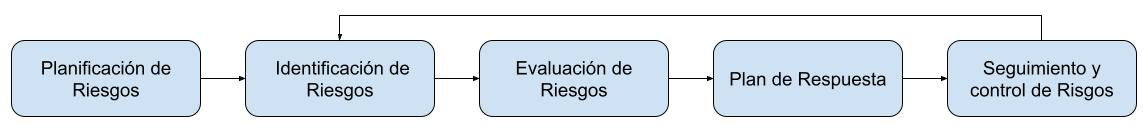
\includegraphics[width=0.8\textwidth]{../imagenes/secciones/6-Gestion-del-proyecto/Proceso de gestion de riesgos.jpg}
    \caption{Etapas del proceso de gestión de riesgos}
    \label{fig:etapasDelProcesoDeGestionDeRiesgos}
\end{figure}

\subsection{Planificación de riesgos}\label{subsec:planificacionDeRiesgos}

Se realizó al principio del proyecto, la cual dio origen al actual documento donde definimos las técnicas, herramientas y momentos donde 
debemos hacer el seguimiento y control que será de forma iterativa para identificar constantemente nuevos riesgos a medida que se van 
manifestando y ajustar aquellos previamente encontrados. 

\begin{itemize}
    \item Se decidió gestionar solamente aquellos riesgos cuya consecuencia fuera negativa para el proyecto.
    \item Se define usar el formato “Matriz de Riesgos del Proyecto” provisto por la software factory de ORT.
    \item La frecuencia para evaluar los riesgos será mensual.
    \item Las categorías de los riesgos serán las siguientes:
    \begin{itemize}
        \item \textbf{Tecnológicos:} relacionados a las tecnologías, codificación, conocimiento técnico, utilización de frameworks y librerías externas.
        \item \textbf{Cliente:} asociados a las decisiones del cliente y su colaboración.
        \item \textbf{Organizacional:} relacionados con el equipo de trabajo, la organización y la comunicación.
        \item \textbf{Gestión:} vinculados a la planificación, seguimiento y gestión del proyecto.
        \item \textbf{Producto y dominio:} asociados a la complejidad del dominio que impactan al producto y su calidad.
\end{itemize}
\end{itemize}

\subsection{Identificación de riesgos}\label{subsec:identificacionDeRiesgos}

Constituye el proceso de detectar posibles eventos o condiciones que puedan tener un impacto negativo en los objetivos del proyecto. Para identificar los 
mismos el equipo realizó una lluvia de ideas para cada categoría y se identifican los riesgos en la Matriz de Riesgos, donde se le asigna un id correspondiente 
a la categoría en la tabla de riesgos. Este indicador permite que cada riesgo asociado a una tarea, proceso, procedimiento o producto pueda ser monitoreado 
adecuadamente. 

% [cita lluvia de ideas: https://riskstorming.com/]
% [link a matriz de riesgos: https://docs.google.com/spreadsheets/d/19ZE0J4PxdwMmAOT_rJ9xxUBOhFSJlKFEvN7BwqIjjrw/edit?usp=sharing]

\subsection{Evaluación de Riesgos}\label{subsec:evaluacionDeRiesgos}

Una vez concluída la identificación de los riesgos se procederá a evaluar su probabilidad de ocurrencia e impacto en el proyecto.

% insertar una tabla de 6x2

\begin{table}[H]
    \centering
    \begin{tabular}{c c}
    \hline
    \textbf{Valor} & \textbf{Impacto} \\ \hline
    1 & Marginal \\ \hline
    2 & Poco importante \\ \hline
    3 & Importante (puede retrasar o adelantar el proyecto) \\ \hline
    4 & Crítica (puede detener el proyecto) \\ \hline
    5 & Catastrófica (fracaso del proyecto) \\ \hline
    \end{tabular}
    \caption{Escala de impacto de riesgos}
    \label{tab:escalaDeImpactoDeRiesgos}
\end{table}


\begin{table}[H]
    \centering
    \begin{tabular}{c c}
    \hline
    \textbf{Valor} & \textbf{Probabilidad} \\ \hline
    1 & No probable \\ \hline
    2 & Poco probable \\ \hline
    3 & Probable \\ \hline
    4 & Muy probable \\ \hline
    5 & Altamente probable \\ \hline
    \end{tabular}
    \caption{Escala de probabilidad de riesgos}
    \label{tab:escalaDeProbabilidadDeRiesgos}
\end{table}

subsubsection{Matriz de magnitud de riesgos}label{subsubsec:matrizDeMagnitudDeRiesgos}

El impacto y la probabilidad definidos anteriormente se combinan en la matriz de riesgos para proporcionar una visualización de 
la magnitud asociada a un riesgo.
La matriz estará dividida en 3 zonas: roja, amarilla y verde, que representan riesgos mayores, moderados y menores respectivamente. 
La zona roja está centrada en la esquina superior derecha de la matriz de riesgo (alto impacto y alta probabilidad), mientras que la 
zona verde está centrada en la esquina inferior izquierda (bajo impacto y baja probabilidad). 

\begin{figure}[H]
    \centering
    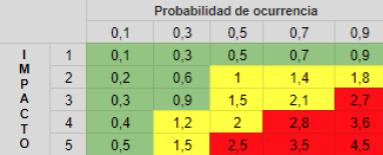
\includegraphics[width=0.8\textwidth]{../imagenes/secciones/6-Gestion-del-proyecto/matriz de riesgos.jpg}
    \caption{Matriz de riesgos}
    \label{fig:matrizDeRiesgos}
\end{figure}

\subsection{Plan de Respuesta}\label{subsec:planDeRespuesta}

Para cada riesgo asignado a un área de la matriz anterior se establecerá una estrategia para su manejo, siendo una de las siguientes:

\begin{itemize}
    \item \textbf{Evitar:} Implica realizar cambios para prevenir que el riesgo ocurra (rojo)
    \item \textbf{Mitigar:} Tomar acciones necesarias para reducir la probabilidad de ocurrencia del riesgo o minimizar su impacto 
    en el proyecto (rojo, amarillo)
    \item \textbf{Transferir:} Compartir el riesgo con el cliente (amarillo, verde)
    \item \textbf{Aceptar:} En algunos casos, especialmente cuando las acciones de mitigación no son efectivas o son muy costosas 
    en términos de tiempo, se podrá optar por aceptar estos riesgos y planificar respuestas contingentes (verde)
    \item \textbf{Monitorear:} Estos riesgos se mantienen bajo observación para detectar cualquier cambio en su estatus (verde, amarillo)
\end{itemize}

\subsection{Seguimiento y Control de riesgos}\label{subsec:monitoreoYControl}

El objetivo de ejecución periódica es monitorear los riesgos con la frecuencia adecuada y considerar las acciones correctivas necesarias 
lo más tempranamente posible intentando minimizar el costo de su implementación.Todos los riesgos irán siendo analizados frecuentemente 
con el objetivo de obtener la evolución de cada riesgo a lo largo del tiempo.

[TODO: insertar una referencia al anexo de la matriz de control de riesgos]